\documentclass{beamer}

\usetheme[progressbar=frametitle]{metropolis}
\setbeamertemplate{frame numbering}[fraction]
\useoutertheme{metropolis}
\useinnertheme{metropolis}
\usefonttheme{metropolis}
\usecolortheme{spruce}
\setbeamercolor{background canvas}{bg=white}

%\usetheme{Warsaw}
%\usecolortheme{crane}
\definecolor{mygray}{rgb}{0.3,0.3,0.3}
\usecolortheme[named=mygray]{structure}


\title[Reinforcement Learning]{Multi-Armed Bandit for Solving Quadratic Assignment Problem}
\subtitle{Reinforcement Learning}
\author{Milad Khademi Nori}
%\institute{Google}
\date{\today}
\begin{document}

\begin{frame}
\titlepage
\end{frame}


\begin{frame}[t]{Contents} %\vspace{10pt}
\begin{enumerate}
\item Introduction to Reinforcement Learning
		\begin{itemize}
		\item Origin \& Goals		
		\item Reinforcement Learning vs Supervised Learning		
		\item Exploration vs Exploitation		
		\item A Single State Example
		\end{itemize}		
\item Multi-Armed Bandit (MAB)
		\begin{itemize}		
		\item Problem Statement
			\begin{itemize}
			\item Epsilon Greedy		
			\item Upper Convergence Bound
			\end{itemize}
		\end{itemize}		
\item Quadratic Assignment Problem (QAB)
		\begin{itemize}
		\item Problem Statement		
			\begin{itemize}		
			\item MAB for Solving QAB			
			\end{itemize}
		\end{itemize}
\end{enumerate}
\end{frame}


\begin{frame}[t]{Introduction to Reinforcement Learning} %\vspace{10pt}
\begin{itemize}
\item Origin
	\begin{itemize}
	\item "A gazelle calf struggles to its feet minutes after being born. Half an hour later it is running at 20 miles per hour." Sutton and Barto
	\end{itemize}
\end{itemize}
\begin{center}
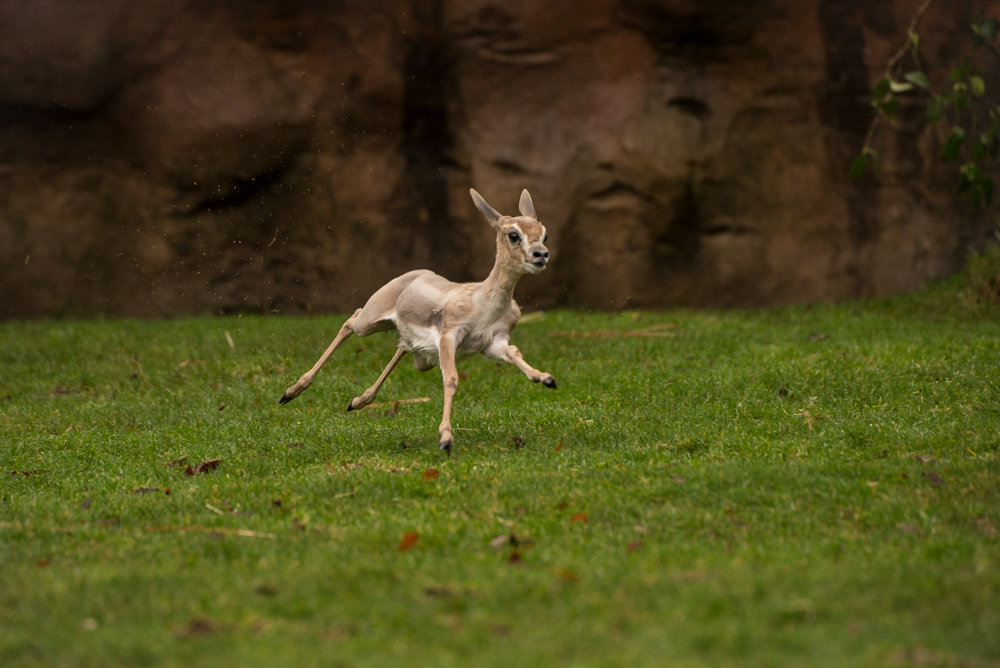
\includegraphics[scale=0.20]{baby}
\end{center}
\end{frame}


\begin{frame}[t]{Introduction to Reinforcement Learning} %\vspace{10pt}
\begin{itemize}
\item Goals
	\begin{itemize}
	\item Agents interacts dynamically with its environment, moves from one state to another.
	\item Based on the actions taken by the agent, rewards are given.
	\item Guidelines for which action to take in each state is called a policy.
	\item Try to efficiently find an optimal policy in which rewards are maximized.
	\end{itemize}
\item Achievement
	\begin{itemize}
	\item Google's AlphaGo used deep reinforcement learning in order to defeat world champion Lee Sedol at Go. In Go number of possible games is larger than the number of atoms in the universe and it is much more challenging than chess.
	\end{itemize}
\end{itemize}
\end{frame}



\begin{frame}[t]{Introduction to Reinforcement Learning} %\vspace{10pt}
\textbf{Reinforcement Learning vs Supervised Learning}
\begin{itemize}
\item Supervised Learning
	\begin{itemize}
	\item Learning from examples (Dataset) provided by knowledgeable external supervisor.
	\item For any state that the agent may be in, the supervisor can supply enough relevant examples of the outcomes which result from similar states so that we may make an accurate prediction.
	\end{itemize}
\item Reinforcement Learning
	\begin{itemize}
	\item No supervisor exists.
	\item Agent must learn from experience as it explore the range of possible states.
	\end{itemize}
\end{itemize}
\end{frame}


\begin{frame}[t]{Introduction to Reinforcement Learning} %\vspace{10pt}
\textbf{Reinforcement Learning vs Supervised Learning}
\begin{itemize}
\item Supervised Learning
	\begin{itemize}
	\item Learning from examples (Dataset) provided by knowledgeable external supervisor.
	\item For any state that the agent may be in, the supervisor can supply enough relevant examples of the outcomes which result from similar states so that we may make an accurate prediction.
	\end{itemize}
\item Reinforcement Learning
	\begin{itemize}
	\item No supervisor exists.
	\item Agent must learn from experience as it explore the range of possible states.
	\end{itemize}
\end{itemize}
\end{frame}


\begin{frame}[t]{Introduction to Reinforcement Learning} %\vspace{10pt}
\begin{itemize}
\item Reinforcement Learning
\end{itemize}
\begin{center}
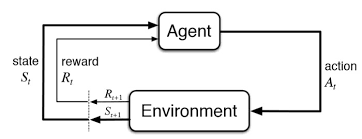
\includegraphics[scale=0.40]{rein}
\end{center}
\begin{itemize}
\item Examples
\end{itemize}
\begin{center}
\resizebox{\textwidth}{!}{
\begin{tabular}{|c c c c c|} 
\hline
\textbf{Agent} & \textbf{Environment} & \textbf{Actions} & \textbf{Rewards} & \textbf{Policy}\\ 
\hline
Board game player & Set of all game configs. & Legal & Winning the game & Optimal strategy\\
Mouse & Maze & Running \& turning & Cheese & Most direct path to cheese\\
\hline
\end{tabular}}
\end{center}
\end{frame}


\begin{frame}[t]{Introduction to Reinforcement Learning} %\vspace{10pt}
\begin{itemize}
\item Exploration \& Exploitation
	\begin{itemize}
	\item In the absence of a supervisor, the agent must explore the environment in order to gain information about rewards, while exploiting its current information to maximize its rewards.
	\item Balancing this tradeoff is a common theme
	\end{itemize}
\item A Single State Example: Multi-Armed Bandit Problem
\end{itemize}
\begin{center}
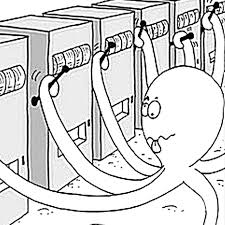
\includegraphics[scale=0.45]{multi}
\end{center}
\end{frame}

\begin{frame}[t]{Multi-Armed Bandit (MAB) Problem} %\vspace{10pt}
\begin{itemize}
\item Multi-Armed Bandit Problem
	\begin{itemize}
	\item Given N different arms to choose from, each with an unknown reward, what strategy should we use to explore and learn the values of each arm, while exploiting our current knowledge to maximize profit?
	\item This is a very common approach for optimizing online marketing campaigns.
	\item This can be thought of as a single-state reinforcement learning problem.
	\end{itemize}
\item MAB Solvers
	\begin{itemize}
	\item Epsilon Greedy
	\item Upper Convergence Bound (UCB)
	\end{itemize}
\end{itemize}			
\end{frame}


\begin{frame}[t]{Multi-Armed Bandit (MAB) Problem} %\vspace{10pt}
\begin{itemize}
\item Upper Convergence Bound (UCB)
\end{itemize}
\begin{equation}
Score_{j}^{t}=\bar{x}_{j}^{t}+\sqrt{\frac{c\times ln\sum_{k}p_{k}^{t}}{p_{j}^{t}}}
\end{equation}
\footnotesize
\begin{itemize}
\item  The first term in the formula, $\bar{x}_{j}^{t}$, encodes the expected average reward for arm $j$ according to knowledge available in time-step $t$.
\item Always choosing the arm with the highest expected reward would result in a purely exploitative algorithm, so the formula includes a second term to deal with exploration.
\item The variable $p_{j}^{t}$ represents the number of times arm $j$ has been pulled at time-step $t$, making the value of the second term in formula inversely proportional to the arm popularity.
\end{itemize}
\end{frame}

\begin{frame}[t]{Quadratic Assignment Problem (QAB)} %\vspace{10pt}
\small
\begin{itemize}
\item The quadratic assignment problem (QAB) is a combinatorial optimization problem introduced by Koopmans and Beckmann in 1957 as a formal model for allocating economical facilities.
\item There are a number of facilities to assign to the same number of locations in an optimal way.
\item A mutual distance is given between locations.
\item Also, a mutual flow is given between facilities which quantifies the mutual interaction between facilities.
\item The aim is to minimize the cost function.
\item The QAP has been proven to be NP-hard ($N!$ solutions).
\end{itemize}
\end{frame}



\begin{frame}[t]{Quadratic Assignment Problem (QAB)} %\vspace{10pt}
\tiny
\begin{equation}
D=
\left[ \begin{array}{ll}
d_{11} \quad \cdots \quad d_{1N}\\
d_{21} \quad \cdots \quad d_{2N}\\
\vdots  \quad \quad \ddots \quad \quad \vdots\\
d_{N1}  \quad \cdots \quad d_{NN}
\end{array} \right],
F=
\left[ \begin{array}{ll}
f_{11} \quad \cdots \quad f_{1N}\\
f_{21} \quad \cdots \quad f_{2N}\\
\vdots  \quad \quad \ddots \quad \quad \vdots\\
f_{N1}  \quad \cdots \quad f_{NN}
\end{array} \right], \quad
d_{11},f_{11}=d_{22},f_{22}=\cdots=d_{NN},f_{NN}=0
\end{equation}
\begin{equation}
\pi()=[\pi(1) \quad \pi(2) \quad \cdots \quad \pi(N)], \quad
1 \leq \pi(1),\pi(2),\cdots,\pi(N) \leq N, \quad
cost(\pi)=\sum_{i=1}^{N}\sum_{j=1}^{N}f_{ij}d_{\pi(i)\pi(j)}
\end{equation}
\begin{center}
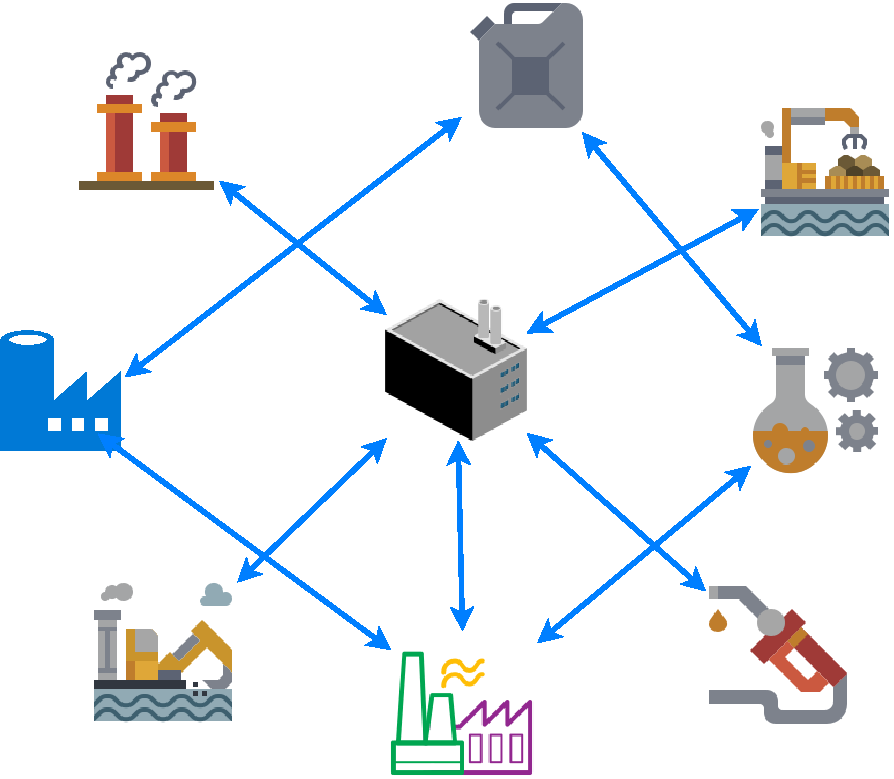
\includegraphics[scale=0.3]{Fac}
\end{center}
\end{frame}

\begin{frame}[t]{MAB for Solving QAB} %\vspace{10pt}
\footnotesize
\begin{center}
\begin{tabular}{ l }
$Population(rnd)\leftarrow\{\pi_{1}^{rnd},\pi_{2}^{rnd},\cdots,\pi_{ps}^{rnd}\}$\\ 
$Populaion(0)\leftarrow LOCAL\_SEARCH(Population(rnd))$\\  
\textbf{Repeat}\\
$A^t\leftarrow SELECT\_SUBSET(Population(t))$\\
$\pi_{i}^{tmp}\leftarrow BUILD\_SOLUTION(A^t,\pi_{i}^{t})$\\
$\pi_{i}^{new}\leftarrow LOCAL\_SEARCH(\pi_{i}^{tmp})$\\  

\textbf{Until}
\end{tabular}
\end{center}
\end{frame}





\end{document}